Cluster analysis and similarity search play a crucial role in identifying patterns in molecular structures and predicting their properties. Consequently, they are among the most commonly used methods of \emph{in silico} studies exploring the structure-activity relationship of chemical compounds. In such context, under the assumption that the similarity between compounds is proportional to~the similarity of their numerical representation, the similarity search can be effectively performed as a KNN-search in the feature space \cite{weber1998knn}. This process is computationally expensive, particularly when operating on high-dimensional representations such as molecular fingerprints. The nearest neighbour similarity search, therefore, serves as an apt validation test for the practical applicability of dimensionality reduction techniques like Johnson-Lindenstrauss and MinHash, which aim to~reduce computational costs without sacrificing accuracy.

The goal is to reduce the likelihood of a false negative, i.e. rejecting a potential neighbour that would be selected based on the original, non-reduced encoding. An error of this kind is more costly than a false positive because it excludes from further study a compound that could potentially be~a~good candidate for the desired active ingredient. The assumption is that the nearest-neighbour search method itself does not use an approximation algorithm and always returns the correct result. In addition, in the context of this problem, instead of similarity, the Jaccard distance (see~\hyperref[ch:notation]{Notation}) will be used, which is directly related to the similarity and follows the convention used for the KNN search. This analysis refers to the MinHash reduction, which has proven to be~the best experimentally and has the desired theoretical properties.

For the analysis, the Jaccard distance distribution for the random set and hydrocarbons can be modelled with a normal distribution.
\begin{figure}[H]
    \centering
    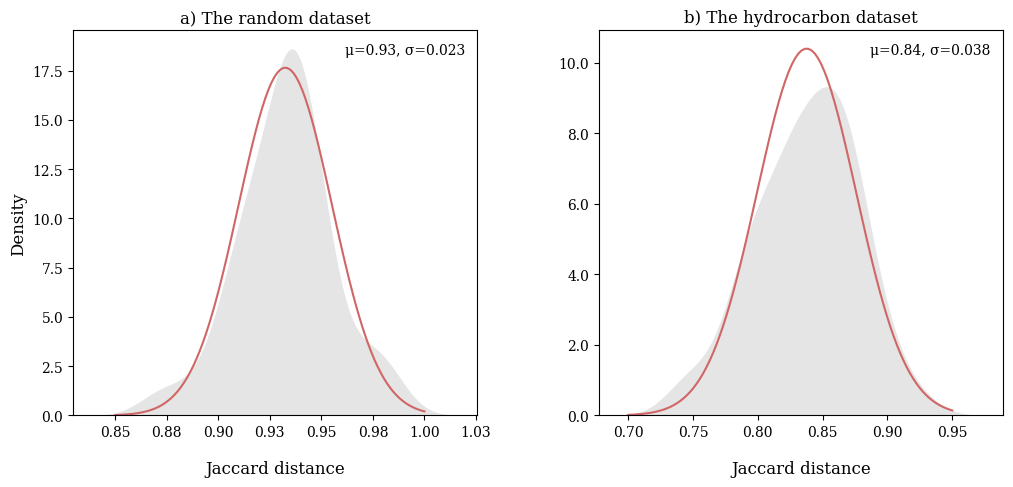
\includegraphics[height=6cm]{figures/similarity_distributions_only.png}
    \caption{Fit of normal distribution to distribution of Jaccard distance}
    \label{fig:normal}
\end{figure}
The problem has two variants: searching for exactly \( k \) nearest neighbours or searching for all neighbours with a distance of at most \( k \) from the input structure. Let \( E \) be an event that a vector \( v \) is included in the results of the search based on the original encoding, and let \( \tilde{E} \) denote the event that \( \tilde{v} = f(v) \) is included in the results of the search based on the reduced encoding. Let \( u \) be the encoding of a given input structure. Suppose we search in a set of \( m \) structures with \( N \) being the maximum number of identifiers generated by the ECFP algorithm. The reduced encoding has length \( n = \bigO(\log(m)\eps^{-2}) \), as in the Lemma~\ref{propos:MH}.

\subsection{Search with fixed distance threshold}
We are given the initial structure \( u \) and the distance threshold \( 0 < k < 1 \). The probability of~observing a false negative is:
\[
    P(\neg \tilde{E} \mid E) = P(d(\tilde{u}, \tilde{v}) > k \mid d(u, v) \leq k)
\]
Since the size of the set of ECFP identifiers for each structure is limited linearly from the size of the structure, the distances between structures take on values from a specific discrete range \linebreak \( D \subseteq \set{\frac{\abs{u \:\cap\: v}}{\abs{u \:\cup\: v}} \colon 0 \leq \abs{u \cap v} \leq N,\; 0 < \abs{u \cup v} \leq 2N} \). Hence, the above probability can be bounded by iterating over all possible distances between \( u \) and \( v \) that are not greater than \( k \):
\[
    P(\neg \tilde{E} \mid E) = \sum_{d_i \in D,\; d_i \leq k}\; P(d(\tilde{u}, \tilde{v}) > d(u, v) + (k - d_i) \mid d(u, v) = d_i) \cdot P(d(u, v) = d_i)
\]
For the MinHash method, we can bound the probability using the Proposition~\ref{propos:MH} and the fact that the distribution of Jaccard distance can be approximated using a normal distribution \( \mathcal{N}(\mu, \sigma^2) \) fitted for the used datasets, to obtain:
\[
    P(\neg \tilde{E} \mid E) \leq \sum_{d_i \in D}\; 2e^{-n(k-d_i)^2} \cdot \frac{1}{\sqrt{2 \pi} \sigma} e^{-\frac{(d_i - \mu)^2}{2\sigma^2}} = \sum_{d_i \in D}\; 2e^{-n(k-d_i)^2} \cdot \frac{1}{\sqrt{2 \pi} \sigma} e^{-\frac{(d_i - \mu)^2}{2\sigma^2}} 
\]
\[
    = \sqrt{\frac{2}{\pi\sigma^2}} \cdot \sum_{d_i \in D}\; e^{-n(k-d_i)^2-\frac{(d_i - \mu)^2}{2\sigma^2}}
\]
The results obtained experimentally and averaged over 1000 trials are presented in \autoref{tab:knn-distance}.
\begin{table}[ht]
    \centering
    \begin{subtable}[t]{0.45\textwidth}
        \centering
        \caption{The random dataset}
        \begin{tabular}{lccc}
            \toprule
            \( k \) & \( n = 128 \) & \( n = 512 \) & \( n = 2048 \) \\
            \midrule
            0.5 & 0.002 & \( < 0.001 \) & \( < 0.001 \) \\
            0.6 & 0.010 & 0.002 & \( < 0.001 \) \\
            0.7 & 0.033 & 0.001 & \( < 0.001 \) \\
            0.8 & 0.177 & 0.008 & \( < 0.001 \) \\
            0.9 & 0.203 & 0.008 & \( < 0.001 \) \\
            \bottomrule
        \end{tabular}
    \end{subtable}%
    \hfill
    \begin{subtable}[t]{0.45\textwidth}
        \centering
        \caption{The hydrocarbon dataset}
        \begin{tabular}{lccc}
            \toprule
            \( k \) & \( n = 128 \) & \( n = 512 \) & \( n = 2048 \) \\
            \midrule
            0.5 & 0.008 & \( < 0.001 \) & \( < 0.001 \) \\
            0.6 & 0.057 & \( < 0.001 \) & \( < 0.001 \) \\
            0.7 & 0.069 & \( < 0.001 \) & \( < 0.001 \) \\
            0.8 & 0.034 & \( < 0.001 \) & \( < 0.001 \) \\
            0.9 & 0.001 & \( < 0.001 \) & \( < 0.001 \) \\
            \bottomrule
        \end{tabular}
    \end{subtable}
    \caption{Experimental false positive rate in KNN depending on the distance threshold \( k \)}
    \label{tab:knn-distance}
\end{table}


\subsection{Search with fixed number of results}
We are given the initial structure \( u \) and the searched number of nearest neighbours \( k \). Let \( E_j \) represent the probability that \( v \) is the \( j \)-th nearest neighbour of \( u \). The probability of observing a false negative is:
\[
    P(\neg \tilde{E} \mid E) = \frac{P(\neg \tilde{E} \land E)}{P(E)} =  \frac{1}{P(E)} \sum_{j \in [k]} P(\neg \tilde{E} \land E_j)
\]
This can be approximated by the probability that there are at least \( k-j \) vectors that are further from \( u \) than \( v \) when non-reduced but closer after the transformation. For a vector \( v_i \) satisfying the above condition, let \( d_v,\; d_{v_i} \) be respectively the distances of \( v \) and \( v_i \) from \( u \). Let \( d_{uv} \) denote the distance by which \( v \) moves relative to \( u \), that is \( d_{uv} = \abs{d(u, v) - d(\tilde{u}, \tilde{v})} \). The following scenarios are possible:
\begin{itemize}
    \item If \( d(u, v) \leq d(\tilde{u}, \tilde{v}) \) and \( d(u, v_i) \leq d(\tilde{u}, \tilde{v_i}) \), the distance of \( v_i \) from \( u \) must decrease by at~least \( d_{v_i} - d_v + d_{uv} \):
    \[
        P(\abs{d(u, v_i) - d(\tilde{u}, \tilde{v_i})} \geq d_{v_i} - d_v + d_{uv}) \leq 2 e^{-n(d_{v_i} - d_v + d_{uv})^2}
    \]
    \item If \( d(u, v) > d(\tilde{u}, \tilde{v}) \) and \( d(u, v_i) \geq d(\tilde{u}, \tilde{v_i}) \), the distance of \( v_i \) from \( u \) must decrease by at~least \( d_{v_i} - d_v - d_{uv} \):
    \[
        P(\abs{d(u, v_i) - d(\tilde{u}, \tilde{v_i})} \geq d_{v_i} - d_v - d_{uv}) \leq 2 e^{-n(d_{v_i} - d_v - d_{uv})^2}
    \]
    \item If \( d(u, v) > d(\tilde{u}, \tilde{v}) \) and \( d(u, v_i) > d(\tilde{u}, \tilde{v_i}) \), the distance of \( v_i \) from \( u \) must decrease by at~most \( d_{v_i} - d_v + d_{uv} \):
    \[
       P(\abs{d(u, v_i) - d(\tilde{u}, \tilde{v_i})}) \leq d_{v_i} - d_v + d_{uv}) \leq 1 - 2 e^{-n(d_{v_i} - d_v + d_{uv})^2}
    \]
\end{itemize}
Combining the above, and given \( d_v \), \( d_{v_i} \) and \( d_{uv} \), the probability that the transformation introduced an inversion between \( v \) and \( v_i \) with respect to the distance to \( u \) can be bounded by:
\[
    2 e^{-n(d_{v_i} - d_v + d_{uv})^2} + 2 e^{-n(d_{v_i} - d_v - d_{uv})^2} + 1 - 2 e^{-n(d_{v_i} - d_v + d_{uv})^2} = 2 e^{-n(d_{v_i} - d_v - d_{uv})^2} + 1
\]
Summing over the possible values of \( d_v \), \( d_{v_i} \) and \( d_{uv} \), we obtain the bound:
\[
    P(d(u, v) < d(u, v_i) \land d(\tilde{u}, \tilde{v}) > d(\tilde{u}, \tilde{v_i})) \leq
\]
\[
    \leq \sum_{d_v \leq d_{v_i} \in D} \pars{P(d(u,v) = d_v, \ d(u, v_i) = d_{v_i}) \cdot \sum_{d_v \in D} P(\abs{d(u, v) - d(\tilde{u}, \tilde{v})} = d_{uv}) \cdot \pars{2 e^{-n(d_{v_i} - d_v - d_{uv})^2} + 1}}
\]
\[
    \leq \sum_{d_v \leq d_{v_i} \in D} \pars{\frac{1}{2 \pi \sigma^2} e^{-\frac{(d_v - \mu)^2 + (d_{v_i} - \mu)^2}{2 \sigma^2}} \cdot \sum_{d_{uv} \in D} \pars{2e^{-nd_{uv}^2} \cdot \pars{2 e^{-n(d_{v_i} - d_v - d_{uv})^2} + 1}}}
\]
\[
    = \frac{1}{\pi \sigma^2} \cdot\!\!\! \sum_{d_v \leq d_{v_i} \in D} \pars{e^{-\frac{(d_v - \mu)^2 + (d_{v_i} - \mu)^2}{2 \sigma^2}} \cdot \sum_{d_{uv} \in D} e^{-nd_{uv}^2} \cdot \pars{2 e^{-n(d_{v_i} - d_v - d_{uv})^2} + 1}}
\]
To simplify the inner sum, the product can be split into two series of the form \( e^{-x^2} \), and then approximated by a Gaussian integral. Let \( c = d_{v_i} - d_v \) for clarity.
\[
    \sum_{d_{uv} \in D} e^{-nd_{uv}^2} \cdot \pars{2 e^{-n(c - d_{uv})^2} + 1} = \sum_{d_{uv} \in D} e^{-n(c - d_{uv})^2 + d_{uv}^2} + \sum_{d_{uv} \in D} e^{-nd_{uv}^2}
\]
The second sum can be directly approximated by the integral, since for sufficiently large \( N \) the~possible values of \( d_{uv} \) are arranged densely.
\[
    \sum_{d_{uv} \in D} e^{-nd_{uv}^2} \approx \int_{D} e^{-nx^2} dx \leq \int_{0}^{+\infty} e^{-nx^2} dx = \frac{1}{2} \sqrt{\frac{\pi}{n}}
\]
The first sum requires simplification, before a similar approximation can be applied. Because \( c \in [0, 1] \), it follows that:
\[
    \sum_{d_{uv} \in D} e^{-nc^2} \cdot e^{2n\pars{d_{uv}c - d_{uv}^2}} = \sum_{d_{uv} \in D} e^{-nc^2} \cdot e^{n\frac{c^2}{2}} \cdot e^{-2n\pars{d_{uv} - \frac{c}{2}}^2} = e^{-n\frac{c^2}{2}} \cdot \sum_{d_{uv} \in D} e^{-2n\pars{d_{uv} - \frac{c}{2}}^2}
\]
\[
     \approx e^{-n\frac{c^2}{2}} \cdot \int_{D} e^{-n\pars{x - \frac{c}{2}}^2} dx \;\leq\; e^{-n\frac{c^2}{2}} \cdot \int_{0}^{+\infty} e^{-n\pars{x - \frac{c}{2}}^2} dx \;\leq\; \frac{1}{2} e^{-n\frac{c^2}{2}} \cdot  \sqrt{\frac{\pi}{n}}
\]
Applying the above derivation, the consequent result is:
\[
    P(\neg \tilde{E} \land E_j) \leq {m-j \choose k-j} \pars{\frac{1}{\pi \sigma^2} \cdot\!\!\! \sum_{d_v \leq d_{v_i} \in D} \pars{e^{-\frac{(d_v - \mu)^2 + (d_{v_i} - \mu)^2}{2 \sigma^2}} \cdot \sqrt{\frac{\pi}{n}} \cdot e^{-n\frac{(d_{v_i} - d_v)^2}{2}}}}^{k-j}
\]
\[
    = {m-j \choose k-j} \pars{\frac{1}{\sqrt{n \pi} \sigma^2} \cdot\!\!\! \sum_{d_v \leq d_{v_i} \in D} \pars{e^{-\frac{(d_v - \mu)^2 + (d_{v_i} - \mu)^2}{2 \sigma^2}} \cdot e^{-n\frac{(d_{v_i} - d_v)^2}{2}}}}^{k-j}
\]
\\

\noindent
The results obtained experimentally over 1000 trials and different threshold values are presented in \autoref{tab:knn-number}.
\begin{table}[ht]
    \centering
    \begin{subtable}[t]{0.45\textwidth}
        \centering
        \caption{The random dataset}
        \begin{tabular}{lccc}
            \toprule
            \( k \) & \( n = 128 \) & \( n = 512 \) & \( n = 2048 \) \\
            \midrule
            10 & 0.319 & 0.005 & 0.025 \\
            20 & 0.311 & 0.046 & 0.024 \\
            30 & 0.305 & 0.046 & 0.024 \\
            40 & 0.297 & 0.044 & 0.023 \\
            50 & 0.290 & 0.043 & 0.022 \\
            \bottomrule
        \end{tabular}
    \end{subtable}%
    \hfill
    \begin{subtable}[t]{0.45\textwidth}
        \centering
        \caption{The hydrocarbon dataset}
        \begin{tabular}{lccc}
            \toprule
            \( k \) & \( n = 128 \) & \( n = 512 \) & \( n = 2048 \) \\
            \midrule
            10 & 0.152 & 0.020 & 0.020 \\
            20 & 0.139 & 0.019 & 0.019 \\
            30 & 0.135 & 0.022 & 0.021 \\
            40 & 0.129 & 0.023 & 0.023 \\
            50 & 0.126 & 0.022 & 0.022 \\
            \bottomrule
        \end{tabular}
    \end{subtable}
    \caption{Experimental false positive rate in KNN depending on the count threshold \( k \)}
    \label{tab:knn-number}
\end{table}
% RANDOM number threshold
% n=128, k=5) 0.3326
% n=128, k=10) 0.31870000000000004
% n=128, k=15) 0.3150666666666667
% n=128, k=20) 0.31115000000000004
% n=128, k=25) 0.30668000000000006
% n=128, k=30) 0.30466666666666664
% n=128, k=35) 0.30071428571428566
% n=128, k=40) 0.29745
% n=128, k=45) 0.29373333333333335
% n=128, k=50) 0.29041999999999996
% n=1024, k=5) 0.027600000000000003
% n=1024, k=10) 0.025200000000000004
% n=1024, k=15) 0.025333333333333333
% n=1024, k=20) 0.024549999999999995
% n=1024, k=25) 0.023799999999999998
% n=1024, k=30) 0.0243
% n=1024, k=35) 0.024485714285714288
% n=1024, k=40) 0.022925000000000004
% n=1024, k=45) 0.02335555555555555
% n=1024, k=50) 0.02246
% n=8192, k=5) 0.0268
% n=8192, k=10) 0.0247
% n=8192, k=15) 0.025333333333333333
% n=8192, k=20) 0.0243
% n=8192, k=25) 0.023839999999999997
% n=8192, k=30) 0.024166666666666663
% n=8192, k=35) 0.02442857142857143
% n=8192, k=40) 0.022825
% n=8192, k=45) 0.023199999999999995
% n=8192, k=50) 0.02222

% RANDOM distance threshold
% n=128, k=0.1) 0.0
%  n=128, k=0.2) 0.0
%  n=128, k=0.3) 0.0
%  n=128, k=0.4) 0.0
%  n=128, k=0.5) 0.002
%  n=128, k=0.6) 0.01
%  n=128, k=0.7) 0.033083333333333326
%  n=1024, k=0.1) 0.0
%  n=1024, k=0.2) 0.0
%  n=1024, k=0.3) 0.0
%  n=1024, k=0.4) 0.0
%  n=1024, k=0.5) 0.0
%  n=1024, k=0.6) 0.0
%  n=1024, k=0.7) 0.0

% SIMILAR number threshold
%  n=128, k=5) 0.1678
%  n=128, k=10) 0.15180000000000002
%  n=128, k=15) 0.14486666666666667
%  n=128, k=20) 0.13925
%  n=128, k=25) 0.13748000000000002
%  n=128, k=30) 0.13490000000000005
%  n=128, k=35) 0.13174285714285713
%  n=128, k=40) 0.1291
%  n=128, k=45) 0.12848888888888887
%  n=128, k=50) 0.12624000000000002
%  n=128, k=0.1) 0.0
%  n=128, k=0.2) 0.0
%  n=128, k=0.3) 0.0
%  n=128, k=0.4) 0.0
%  n=128, k=0.5) 0.008
%  n=128, k=0.6) 0.057083333333333326
%  n=128, k=0.7) 0.069225093685548
%  n=1024, k=5) 0.0258
%  n=1024, k=10) 0.020200000000000003
%  n=1024, k=15) 0.02053333333333333
%  n=1024, k=20) 0.0189
%  n=1024, k=25) 0.02084
%  n=1024, k=30) 0.021299999999999996
%  n=1024, k=35) 0.021200000000000004
%  n=1024, k=40) 0.022775000000000007
%  n=1024, k=45) 0.021799999999999996
%  n=1024, k=50) 0.02178
%  n=1024, k=0.1) 0.0
%  n=1024, k=0.2) 0.0
%  n=1024, k=0.3) 0.0
%  n=1024, k=0.4) 0.0
%  n=1024, k=0.5) 0.0
%  n=1024, k=0.6) 0.0
%  n=1024, k=0.7) 0.0
%  n=8192, k=5) 0.0258
%  n=8192, k=10) 0.020200000000000003
%  n=8192, k=15) 0.02053333333333333
%  n=8192, k=20) 0.0189
%  n=8192, k=25) 0.02084
%  n=8192, k=30) 0.021299999999999996
%  n=8192, k=35) 0.021200000000000004
%  n=8192, k=40) 0.022775000000000007
%  n=8192, k=45) 0.021799999999999996
%  n=8192, k=50) 0.02178
%  n=8192, k=0.1) 0.0
%  n=8192, k=0.2) 0.0
%  n=8192, k=0.3) 0.0
%  n=8192, k=0.4) 0.0
%  n=8192, k=0.5) 0.0
%  n=8192, k=0.6) 0.0
%  n=8192, k=0.7) 0.0